\documentclass[../main.tex]{subfiles}
\begin{document}
La cinematica studia il moto dei corpi, non le cause (quello fa parte della dinamica).
Il sistema di riferimento per la cinematica \textbf{unidimensionale} è composto da una sola retta, che possiamo definire a piacere.

\subsection{Moto uniformemente accellerato}
\subsubsection{Distanza e spostamento}
\begin{itemize}
    \item distanza $d \phantom{-} \lbrack m \rbrack$: lunghezza del percorso, sempre $\geq 0$
    \item spostamento $\Delta x$ oppure $\Delta y \phantom{-} \lbrack m\rbrack$: $\Delta x=x_f-x_i$: differenza di posizione
\end{itemize}
\textbf{Nota:} distanza $\neq$ spostamento, la distanza tiene conto del percorso e delle eventuali tappe, è un valore sempre positivo quindi anche se si torna indietro rispetto al sistema di riferimento aumenterà, lo spostamento invece è relativo soltanto a $x_i$ e $x_f$, non tiene conto di eventuali allungamenti di percorso, banalmente se torno mi muovo di 2 metri e ritorno al punto di partenza lo spostamento risulterà 0. Ecco alcuni esempi:

\begin{center}
    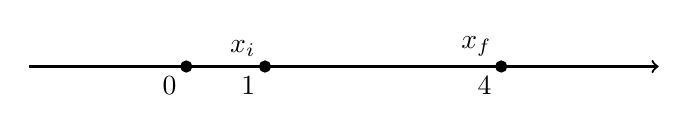
\begin{tikzpicture}
         % Disegna i punti
        \filldraw[black] (0,0) circle (2pt) node[anchor=north east] {0} ;
        \filldraw[black] (1,0) circle (2pt) node[anchor=north east] {1} node[anchor=south east] {$x_i$};
        \filldraw[black] (4,0) circle (2pt) node[anchor=north east] {4} node[anchor=south east] {$x_f$};

         % Definizione dei vettori
        \draw[->, thick, black] (-2,0) -- (6,0) node[midway, below] {};
    \end{tikzpicture}
    
    $d=3m\phantom{---} \Delta x=4-1=3m$
\end{center}
\vspace{1cm}
\begin{center}
    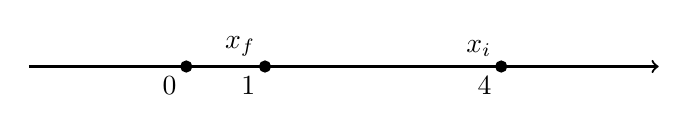
\begin{tikzpicture}
         % Disegna i punti
        \filldraw[black] (0,0) circle (2pt) node[anchor=north east] {0} ;
        \filldraw[black] (1,0) circle (2pt) node[anchor=north east] {1} node[anchor=south east] {$x_f$};
        \filldraw[black] (4,0) circle (2pt) node[anchor=north east] {4} node[anchor=south east] {$x_i$};

         % Definizione dei vettori
        \draw[->, thick, black] (-2,0) -- (6,0) node[midway, below] {};
    \end{tikzpicture}
    
    $d=3m\phantom{---} \Delta x=1-4=-3m$
\end{center}
\vspace{1cm}
\begin{center}
    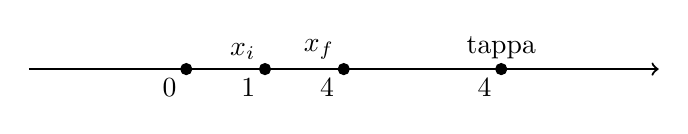
\begin{tikzpicture}
         % Disegna i punti
        \filldraw[black] (0,0) circle (2pt) node[anchor=north east] {0} ;
        \filldraw[black] (1,0) circle (2pt) node[anchor=north east] {1} node[anchor=south east] {$x_i$};
        \filldraw[black] (2,0) circle (2pt) node[anchor=north east] {4} node[anchor=south east] {$x_f$};
        \filldraw[black] (4,0) circle (2pt) node[anchor=north east] {4} node[anchor=south] {tappa};

         % Definizione dei vettori
        \draw[->, thick, black] (-2,0) -- (6,0) node[midway, below] {};
    \end{tikzpicture}
    
    $d=3+2=5m\phantom{---} \Delta x=2-1=1m$
\end{center}

\subsubsection{Velocità}
\begin{itemize}
    \item velocità scalare media $v=\frac{d}{t} \phantom{-} \lbrack \frac{m}{s}\rbrack$: lunghezza del percorso, sempre $\geq 0$
    \item velocità media $v=\frac{\Delta x}{\Delta t} \phantom{-}\lbrack \frac{m}{s}\rbrack$: può essere negativa \begin{align*}
        v&=\frac{x_f-x_i}{t_f-t_i} \\
        &=\frac{x_f-x_i}{t} \text{ con } t_i=0s
    \end{align*}
    \item velocità istantanea $v_i=\lim\limits_{\Delta t \to 0}\frac{\Delta x}{\Delta t}$
\end{itemize}
\textbf{Nota:} nella velocità istantanea $\Delta t$ è tendente a 0, si calcola quindi la pendenza della retta tangente (la formula è uguale a quella della velocità media solo che $\Delta t$ tende a $0$.

\subsubsection{Accellerazione}
\begin{itemize}
    \item accellerazione media $a_m=\frac{\Delta v}{\Delta t} \phantom{-} \lbrack \frac{m}{s}\rbrack$
    \item accellerazione istantanea $a_i=\lim\limits_{\Delta t \to 0}a_m$, vale lo stesso discorso della velocità istantanea
\end{itemize}

\subsubsection{Leggi del moto}
Per riassumere, ecco una lista delle formule utili, in questo documento non sono svolte le dimostrazioni:
\begin{itemize}
    \item $V_f = V_i + a \cdot t$ (è un equazione affine, una retta), \textbf{legge della velocià}
    \item $V_m = \frac{1}{2}(V_i+V_f)$, \textbf{velocità media}
    \item $x_f = x_i + \frac{V_i + V_f}{2} \cdot t$, \textbf{posizione in funzione della velocità media}
    \item $x_f = x_i + V_i \cdot t + \frac{1}{2} \cdot a \cdot t^2$, \textbf{posizione in funzione della velocità iniziale e dell'accellerazione}
    \item $V_f^2 = V_i^2 + 2 \cdot a \cdot \Delta x$, la formula generale dalla quale si ricavano le altre
\end{itemize}
\textbf{Nota:} in molte situazioni il tempo iniziale non viene indicato perchè si da scontato che sia $0$.
Inoltre spesso quando troviamo $V$, si parla di $V_f$.

\subsection{Moto di caduta}
Il moto di caduta è il moto in cui il corpo è soggetto alla forza di gravità vale che
$$
    \Vert \vec{g} \Vert = 9.81 \frac{m}{s^2}
$$
in base al sistema di riferimento scelto.

\subsubsection{Caduta libera}
Prendiamo come base un sistema di riferimento dove $g$ è \textbf{positivo}.
\begin{itemize}
    \item $t = \sqrt{\frac{2y}{g}}$, il tempo di caduta
    \item $g = \frac{V}{t}$
    \item $V = g \cdot t = \sqrt{2 g y}$, velocità ottenuta dopo $y$ metri
\end{itemize}

\subsubsection{Lancio verso l'alto}
In questo caso usiamo un sistema di riferimento dove $g$ è \textbf{negativo}.
\begin{itemize}
    \item $t = \frac{2 \cdot V_0}{g}$, il tempo di volo
    \item $V_0 = \frac{1}{2}gt$
    \item $V = -V_0$
\end{itemize}

\begin{center}
    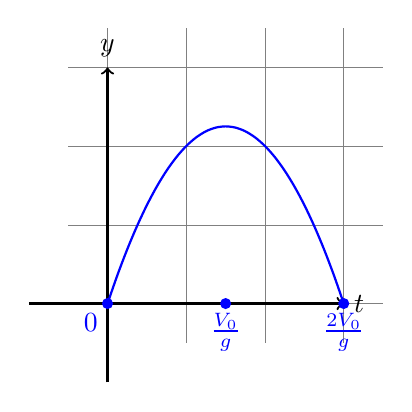
\begin{tikzpicture}
        % Disegna la griglia
        \draw[very thin, gray] (-0.5,-0.5) grid (3.5,3.5);
        
        % Disegna assi
        \draw[thick,->] (-1,0) -- (3,0) node[right] {$t$}; % Asse x
        \draw[thick,->] (0,-1) -- (0,3) node[above] {$y$}; % Asse y

        % Disegna la funzione y = 3x - 2
        \draw[domain=0:3,smooth,variable=\x,blue,thick] 
        plot (\x, {-(\x)^2+3*(\x)+0}) node[above] {};

        \fill[blue] (3, 0) circle (2pt) node[below] {$\frac{2V_0}{g}$}; % Pallino spesso
        \fill[blue] (1.5, 0) circle (2pt) node[below] {$\frac{V_0}{g}$}; % Pallino spesso
        \fill[blue] (0, 0) circle (2pt) node[below left] {$0$}; % Pallino spesso


    \end{tikzpicture} \hspace{0.3cm}
    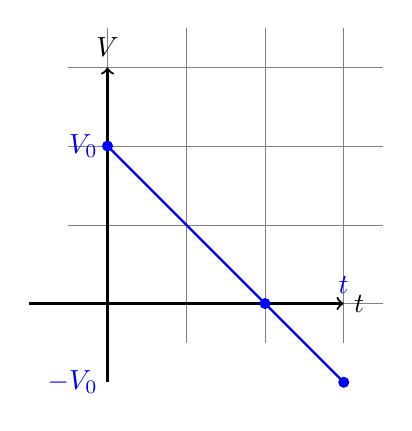
\begin{tikzpicture}
        % Disegna la griglia
        \draw[very thin, gray] (-0.5,-0.5) grid (3.5,3.5);
        
        % Disegna assi
        \draw[thick,->] (-1,0) -- (3,0) node[right] {$t$}; % Asse x
        \draw[thick,->] (0,-1) -- (0,3) node[above] {$V$}; % Asse y

        % Disegna la funzione y = 3x - 2
        \draw[domain=0:3,smooth,variable=\x,blue,thick] 
        plot (\x, {-(\x)+2}) node[above] {};

        \fill[blue] (0, 2) circle (2pt) node[left] {$V_0$}; % Pallino spesso
        \fill[blue] (2, 0) circle (2pt) node[below] {}; % Pallino spesso
        \fill[blue] (3, -1) circle (2pt) node[below] {}; % Pallino spesso

        \node[blue] at (0, -1) [left] {$-V_0$}; % Etichetta sotto
        \node[blue] at (3, 0) [above] {$t$}; % Etichetta sotto
    \end{tikzpicture} \hspace{0.3cm}
    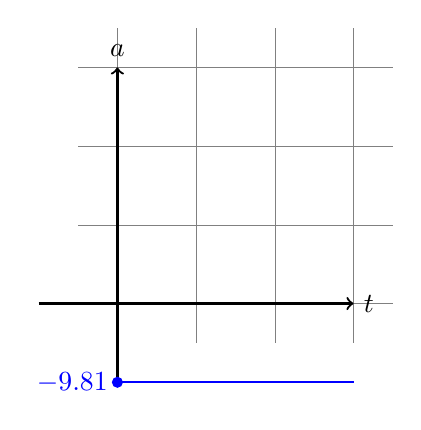
\begin{tikzpicture}
        % Disegna la griglia
        \draw[very thin, gray] (-0.5,-0.5) grid (3.5,3.5);
        
        % Disegna assi
        \draw[thick,->] (-1,0) -- (3,0) node[right] {$t$}; % Asse x
        \draw[thick,->] (0,-1) -- (0,3) node[above] {$a$}; % Asse y

        % Disegna la funzione y = 3x - 2
        \draw[domain=0:3,smooth,variable=\x,blue,thick] 
        plot (\x, {-1}) node[left] {};

        \fill[blue] (0, -1) circle (2pt) node[left] {$-9.81$}; % Pallino spesso
    \end{tikzpicture}
\end{center}
\textbf{Nota:} Nel primo grafico il tempo di salita è uguale al tempo di discesa (in un sistema senza attrito e quindi non nella vita reale).

\subsubsection{Considerazioni sui grafici}
$$
    x = \color{blue}x_0 \color{black}+ \color{green}V_{tot} \color{black}+ \color{red}\frac{1}{2}a\color{black}t^2\longleftrightarrow y=\color{red}a\color{black}x^2+bx+\color{blue}c\color{black}
$$
\color{blue}$x_0$ \color{black}è il termine noto, \color{green}$V_{tot}$\color{black} è la pendenza della retta tangente nel punto iniziale,
\color{red}$\frac{1}{2}a$ \color{black} è la concavità.

Ecco alcuni esempi:
\begin{center}
    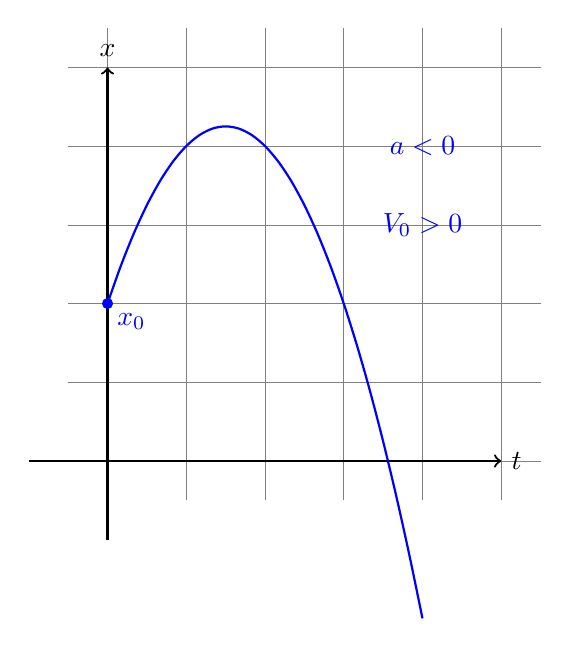
\begin{tikzpicture}
        % Disegna la griglia
        \draw[very thin, gray] (-0.5,-0.5) grid (5.5,5.5);
        
        % Disegna assi
        \draw[thick,->] (-1,0) -- (5,0) node[right] {$t$}; % Asse x
        \draw[thick,->] (0,-1) -- (0,5) node[above] {$x$}; % Asse y

        % Disegna la funzione y = 3x - 2
        \draw[domain=0:4,smooth,variable=\x,blue,thick] 
        plot (\x, {-(\x)^2+3*(\x)+2}) node[above] {};

        \fill[blue] (0, 2) circle (2pt) node[below right] {$x_0$}; % Pallino spesso

        \node[blue] at (4, 4) {$a<0$}; % Etichetta sotto
        \node[blue] at (4, 3) {$V_0>0$}; % Etichetta sotto
    \end{tikzpicture} \hspace{1cm}
    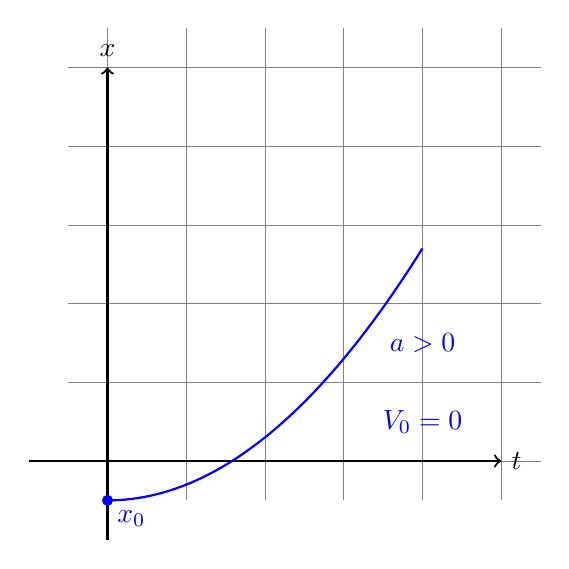
\begin{tikzpicture}
        % Disegna la griglia
        \draw[very thin, gray] (-0.5,-0.5) grid (5.5,5.5);
        
        % Disegna assi
        \draw[thick,->] (-1,0) -- (5,0) node[right] {$t$}; % Asse x
        \draw[thick,->] (0,-1) -- (0,5) node[above] {$x$}; % Asse y

        % Disegna la funzione y = 3x - 2
        \draw[domain=0:4,smooth,variable=\x,blue,thick] 
        plot (\x, {0.2*(\x^2)-0.5}) node[above] {};

        \fill[blue] (0, -0.5) circle (2pt) node[below right] {$x_0$}; % Pallino spesso

        \node[blue] at (4, 1.5) {$a>0$}; % Etichetta sotto
        \node[blue] at (4, 0.5) {$V_0=0$}; % Etichetta sotto
    \end{tikzpicture}
\end{center}

\begin{center}
    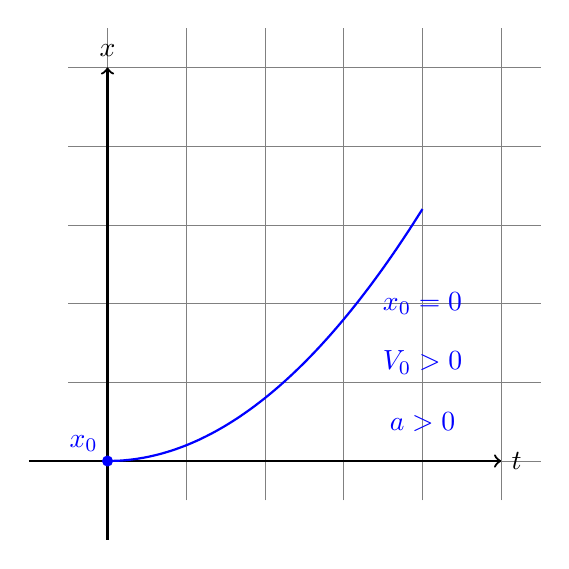
\begin{tikzpicture}
        % Disegna la griglia
        \draw[very thin, gray] (-0.5,-0.5) grid (5.5,5.5);
        
        % Disegna assi
        \draw[thick,->] (-1,0) -- (5,0) node[right] {$t$}; % Asse x
        \draw[thick,->] (0,-1) -- (0,5) node[above] {$x$}; % Asse y

        % Disegna la funzione y = 3x - 2
        \draw[domain=0:4,smooth,variable=\x,blue,thick] 
        plot (\x, {0.2*(\x^2)}) node[above] {};

        \fill[blue] (0, 0) circle (2pt) node[above left] {$x_0$}; % Pallino spesso

        \node[blue] at (4, 2) {$x_0=0$}; % Etichetta sotto
        \node[blue] at (4, 1.25) {$V_0>0$}; % Etichetta sotto
        \node[blue] at (4, 0.5) {$a>0$}; % Etichetta sotto

    \end{tikzpicture} \hspace{1cm}
    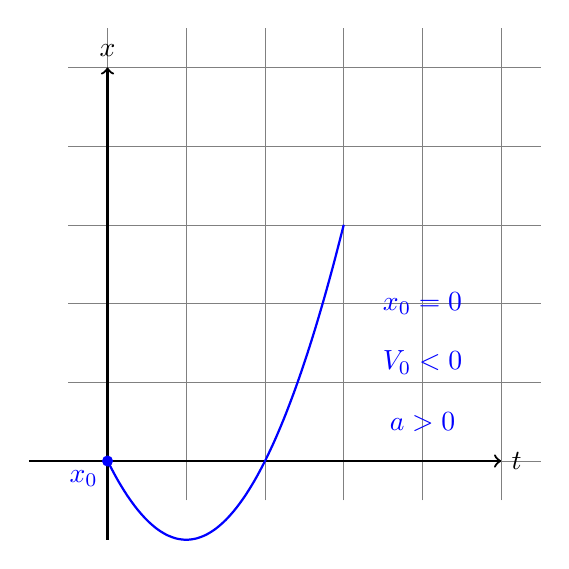
\begin{tikzpicture}
        % Disegna la griglia
        \draw[very thin, gray] (-0.5,-0.5) grid (5.5,5.5);
        
        % Disegna assi
        \draw[thick,->] (-1,0) -- (5,0) node[right] {$t$}; % Asse x
        \draw[thick,->] (0,-1) -- (0,5) node[above] {$x$}; % Asse y

        % Disegna la funzione y = 3x - 2
        \draw[domain=0:3,smooth,variable=\x,blue,thick] 
        plot (\x, {(\x-1)^2 -1}) node[above] {};

        \fill[blue] (0, 0) circle (2pt) node[below left] {$x_0$}; % Pallino spesso

        \node[blue] at (4, 2) {$x_0=0$}; % Etichetta sotto
        \node[blue] at (4, 1.25) {$V_0<0$}; % Etichetta sotto
        \node[blue] at (4, 0.5) {$a>0$}; % Etichetta sotto
    \end{tikzpicture} 
\end{center}
\end{document}